    \newcommand{\RingSegment}[6]{%
% #1 = center coordinate
% #2 = inner radius
% #3 = outer radius
% #4 = start angle
% #5 = delta angle
% #6 = TikZ style
\fill[#6]
  (#1) ++(#4:#2)
  arc[start angle=#4, delta angle=#5, radius=#2]
  -- ++(#4+#5:#3-#2)
  arc[start angle=#4+#5, delta angle=-#5, radius=#3]
  -- cycle;
}
\newcommand{\RingLabel}[5]{%
% #1 = center coordinate
% #2 = radius
% #3 = start angle
% #4 = delta angle
% #5 = text
  \pgfmathsetmacro{\angTmp}{#3 + 0.5*#4}
  \pgfmathsetmacro{\rotTmp}{\angTmp}
  \pgfmathsetmacro{\rotTmp}{%
      (\angTmp < 240) ? \angTmp + 180 : ((\angTmp < 300) ? \angTmp + 90 : \angTmp)
    }
  \node[
    font=\bfseries\tiny,
    align=center,
    rotate=\rotTmp
  ] at ($ (#1) + (\angTmp:#2) $) {#5};
}
\newcommand{\RingLabelCurved}[5]{%
% #1 = center
% #2 = radius
% #3 = start angle
% #4 = delta angle
% #5 = text
  \pgfmathsetmacro{\aMid}{#3 + 0.5*#4}
  \path[
    decorate,
    decoration={
      text along path,
      text={|\bfseries\scriptsize|#5},
      text align=center,
      raise=0.5ex
    }
  ]
  (#1) ++(#3:#2)
  arc[start angle=#3, delta angle=#4, radius=#2];
}
\newcommand{\InputOutputBox}[7]{%
    \node[align=justify, anchor=#1, text width=#3, minimum width=#3, minimum height=#2, fill=#4, rounded corners=2mm, font=\fontsize{1pt}{1pt}\selectfont] at (#5) 
          {%
              \textbf{Input:} #6\newline
              \textbf{Output:} #7
    };
}


\begin{figure*}[h!tb]
    \centering

    \begin{tikzpicture}        
        \node[anchor=center] (refMap) at (0,0) {};

        % radii: inner just outside image, outer controls thickness
        \def\rInner{0.4*\BenImgWidth}
        \def\rMid{0.85*\BenImgWidth}
        \def\rOuter{1.25*\BenImgWidth}
        \def\lineSep{1pt}
        \pgfmathsetmacro{\rLabelInner}{1.9}
        \pgfmathsetmacro{\rLabelMid}{2.1}
        \pgfmathsetmacro{\rLabelOuter}{2.5}
        
        \def\aStart{90}
        \def\aBin{136.6}
        \def\aBB{83.1}
        \def\aCap{17.5}
        \def\aMCQ{122.8}
        
        % inner segments
        \RingSegment{refMap}{\rInner}{\rMid}{\aStart}{\aBin}{Orchid!42.5, draw=white, line width=\lineSep}
        \RingSegment{refMap}{\rInner}{\rMid}{\aStart+\aBin}{\aBB}{red!37.5,draw=white,line width=\lineSep}
        \RingSegment{refMap}{\rInner}{\rOuter}{\aStart+\aBin+\aBB}{\aCap}{yellow!50,draw=white,line width=\lineSep}
        \RingSegment{refMap}{\rInner}{\rMid}{\aStart+\aBin+\aBB+\aCap}{\aMCQ}{YellowGreen!40,draw=white,line width=\lineSep}
        \RingLabelCurved{refMap}{\rLabelInner}{\aStart}{\aBin}{Binary VQA}
        \RingLabelCurved{refMap}{0.85*\rLabelInner}{\aStart+\aBin}{\aBB}{Ref. Exp.}
        \RingLabelCurved{refMap}{\rLabelInner}{\aStart+\aBin}{\aBB}{Detection}
        \RingLabel{refMap}{\rLabelMid}{\aStart+\aBin+\aBB}{\aCap}{Captioning}
        \RingLabelCurved{refMap}{\rLabelInner}{\aStart+\aBin+\aBB+\aCap}{\aMCQ}{Multiple-Choice VQA}

        \def\bBinAdj{31.8}
        \def\bBinArea{34.9}
        \def\bBinCount{34.9}
        \def\bBinPresence{34.9}
        \RingSegment{refMap}{\rMid}{\rOuter}{\aStart}{\bBinAdj}{Orchid!15, draw=white, line width=\lineSep}
        \RingSegment{refMap}{\rMid}{\rOuter}{\aStart+\bBinAdj}{\bBinArea}{Orchid!30, draw=white, line width=\lineSep}
        \RingSegment{refMap}{\rMid}{\rOuter}{\aStart+\bBinAdj+\bBinArea}{\bBinCount}{Orchid!45, draw=white, line width=\lineSep}
        \RingSegment{refMap}{\rMid}{\rOuter}{\aStart+\bBinAdj+\bBinArea+\bBinCount}{\bBinPresence}{Orchid!60, draw=white, line width=\lineSep}
        \RingLabel{refMap}{\rLabelOuter}{\aStart}{\bBinAdj}{\adjacencyABBR}
        \RingLabel{refMap}{\rLabelOuter}{\aStart+\bBinAdj}{\bBinArea}{\areaABBR}
        \RingLabel{refMap}{\rLabelOuter}{\aStart+\bBinAdj+\bBinArea}{\bBinCount}{\countABBR}
        \RingLabel{refMap}{\rLabelOuter}{\aStart+\bBinAdj+\bBinArea+\bBinCount}{\bBinPresence}{\presenceABBR}
        
        \def\bBBPoint{43.1}
        \def\bBBRef{40.0}
        \RingSegment{refMap}{\rMid}{\rOuter}{\aStart+\aBin}{\bBBPoint}{red!25,draw=white,line width=\lineSep}
        \RingSegment{refMap}{\rMid}{\rOuter}{\aStart+\aBin+\bBBPoint}{\bBBRef}{red!50,draw=white,line width=\lineSep}
        \RingLabel{refMap}{\rLabelOuter}{\aStart+\aBin}{\bBBPoint}{Ref. Point\\Detection}
        \RingLabel{refMap}{\rLabelOuter}{\aStart+\aBin+\bBBPoint}{\bBBRef}{Ref. LULC\\Detection}
        
        \def\bCap{17.5}
        
        \def\bMCQAdj{14.3}
        \def\bMCQArea{17.5}
        \def\bMCQClimate{17.5}
        \def\bMCQCount{17.5}
        \def\bMCQCountry{17.5}
        \def\bMCQPresence{17.5}
        \def\bMCQRelPos{3.7}
        \def\bMCQSeason{17.5}
        \RingSegment{refMap}{\rMid}{\rOuter}{\aStart+\aBin+\aBB+\aCap}{\bMCQAdj}{YellowGreen!10,draw=white,line width=\lineSep}
        \RingSegment{refMap}{\rMid}{\rOuter}{\aStart+\aBin+\aBB+\aCap+\bMCQAdj}{\bMCQArea}{YellowGreen!20,draw=white,line width=\lineSep}
        \RingSegment{refMap}{\rMid}{\rOuter}{\aStart+\aBin+\aBB+\aCap+\bMCQAdj+\bMCQArea}{\bMCQClimate}{YellowGreen!30,draw=white,line width=\lineSep}
        \RingSegment{refMap}{\rMid}{\rOuter}{\aStart+\aBin+\aBB+\aCap+\bMCQAdj+\bMCQArea+\bMCQClimate}{\bMCQCount}{YellowGreen!40,draw=white,line width=\lineSep}
        \RingSegment{refMap}{\rMid}{\rOuter}{\aStart+\aBin+\aBB+\aCap+\bMCQAdj+\bMCQArea+\bMCQClimate+\bMCQCount}{\bMCQCountry}{YellowGreen!50,draw=white,line width=\lineSep}
        \RingSegment{refMap}{\rMid}{\rOuter}{\aStart+\aBin+\aBB+\aCap+\bMCQAdj+\bMCQArea+\bMCQClimate+\bMCQCount+\bMCQCountry}{\bMCQPresence}{YellowGreen!60,draw=white,line width=\lineSep}
        \RingSegment{refMap}{\rMid}{\rOuter}{\aStart+\aBin+\aBB+\aCap+\bMCQAdj+\bMCQArea+\bMCQClimate+\bMCQCount+\bMCQCountry+\bMCQPresence}{\bMCQRelPos}{YellowGreen!70,draw=white,line width=\lineSep}
        \RingSegment{refMap}{\rMid}{\rOuter}{\aStart+\aBin+\aBB+\aCap+\bMCQAdj+\bMCQArea+\bMCQClimate+\bMCQCount+\bMCQCountry+\bMCQPresence+\bMCQRelPos}{\bMCQSeason}{YellowGreen!80,draw=white,line width=\lineSep}
        \RingLabel{refMap}{\rLabelOuter}{\aStart+\aBin+\aBB+\aCap}{\bMCQAdj}{\adjacencyABBR}
        \RingLabel{refMap}{\rLabelOuter}{\aStart+\aBin+\aBB+\aCap+\bMCQAdj}{\bMCQArea}{\areaABBR}
        \RingLabel{refMap}{\rLabelOuter}{\aStart+\aBin+\aBB+\aCap+\bMCQAdj+\bMCQArea}{\bMCQClimate}{\climateABBR}
        \RingLabel{refMap}{\rLabelOuter}{\aStart+\aBin+\aBB+\aCap+\bMCQAdj+\bMCQArea+\bMCQClimate}{\bMCQCount}{\countABBR}
        \RingLabel{refMap}{\rLabelOuter}{\aStart+\aBin+\aBB+\aCap+\bMCQAdj+\bMCQArea+\bMCQClimate+\bMCQCount}{\bMCQCountry}{\countryABBR}
        \RingLabel{refMap}{\rLabelOuter}{\aStart+\aBin+\aBB+\aCap+\bMCQAdj+\bMCQArea+\bMCQClimate+\bMCQCount+\bMCQCountry}{\bMCQPresence}{\presenceABBR}
        \RingLabel{refMap}{\rLabelOuter}{\aStart+\aBin+\aBB+\aCap+\bMCQAdj+\bMCQArea+\bMCQClimate+\bMCQCount+\bMCQCountry+\bMCQPresence}{\bMCQRelPos}{\relativepositionABBR}
        \RingLabel{refMap}{\rLabelOuter}{\aStart+\aBin+\aBB+\aCap+\bMCQAdj+\bMCQArea+\bMCQClimate+\bMCQCount+\bMCQCountry+\bMCQPresence+\bMCQRelPos}{\bMCQSeason}{\seasonABBR}

        \begin{scope}
          \clip[rounded corners=5mm]
            ($(refMap)+(-0.5*\BenImgWidth,-0.5*\BenImgWidth)$)
            rectangle
            ($(refMap)+( 0.5*\BenImgWidth, 0.5*\BenImgWidth)$);
        
          \node[anchor=center, inner sep=0pt] at (refMap)
            %{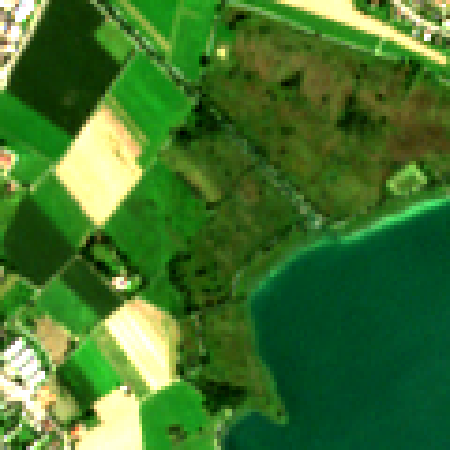
\includegraphics[width=\BenImgWidth]{figures/dataset/samples/_tci_S2A_MSIL2A_20170818T103021_N9999_R108_T32TMT_61_44.png}};
            {\begin{tikzpicture}[scale=0.9]
  % outer disk
  \fill[BlueGreen!20] (0,0) circle (1.2);
  \draw[white, line width=1pt] (0,0) circle (1.2);
  \draw[BlueGreen!50, line width=0.6pt] (0,0) circle (1);

  % latitude / longitude hints
  \draw[BlueGreen!60, line width=0.6pt] (-1.0,0) arc (180:360:1.0 and 0.35);
  \draw[BlueGreen!40, line width=0.3pt, dashed] (-1.0,0) arc (180:0:1.0 and 0.35);
  
  
  \draw[BlueGreen!40, line width=0.3pt, dashed] (0,-1.0) arc (-90:90:0.35 and 1.0);
  \draw[BlueGreen!60, line width=0.6pt] (0,-1.0) arc (-90:-270:0.35 and 1.0);

  
  \draw[BlueGreen!50, line width=0.6pt] (0,0) circle (1);


  % text bars (.txt)
  \node at (-0.6, 0) {
\includegraphics[scale=0.021,decodearray={0 0.65 0 0.65 0 0.65}]{figures/ben_txt_logos/rsim_logo_weiss.png}};
  \fill[gray!70] (-0.2,-0.2) rectangle (0.8,-0.12);
  \fill[gray!70] (-0.2,-0.05) rectangle (0.65,0.03);
  \fill[gray!70] (-0.2,0.10) rectangle (0.75,0.18);

  % name
  %\node[font=\bfseries\scriptsize] at (0,-0.55) {BigEarthNet};
  \path[decorate,decoration={text along path,text={|\bfseries\notsotiny|BigEarthNet},text align=center,raise=-1.6ex}] (-1.0,0) arc (180:360:1.0 and 0.35);
  \node[font=\bfseries\small] at (0,-0.8) {\texttt{.txt}};
\end{tikzpicture}};
        \end{scope}
        
        \def\boxHeight{18mm}
        \def\boxWidth{20mm}  % 20mm
        \InputOutputBox{south east}{0.7*\boxHeight}{\boxWidth}{YellowGreen!60}{$(-\rOuter, -\rOuter) + (-.1,0)$}{Which season is shown in the satellite image? a)~Spring, b)~Summer, c)~Winter, d)~Autumn}{b}
        \InputOutputBox{north east}{0.7*\boxHeight}{\boxWidth}{Orchid!60}{$(-\rOuter, 0) + (-.1,-.05)$}{Are there regions of coastal wetlands in the satellite image?}{No}
        \InputOutputBox{south east}{0.7*\boxHeight}{\boxWidth}{Orchid!15}{$(-\rOuter, 0) + (-.1,.05)$}{Does any inland water border inland wetlands in this scene?}{Yes}
        \InputOutputBox{north east}{0.86*\boxHeight}{\boxWidth}{YellowGreen!40}{$(-\rOuter, \rOuter) + (-.1,0)$}{How many areas covered by urban fabric can be seen? a)~More than five, b)~3, c)~1, d)~0}{b}
        
        \InputOutputBox{south west}{\boxHeight}{\boxWidth}{red!25}{$(\rOuter, -\rOuter) + (.1,-.1)$}{Output a bounding box enclosing the land cover class instance positioned at <point>(0.83, 0.06)</point>.}{[0.49 0.0, 1.0 0.2]}
        \InputOutputBox{west}{\boxHeight}{\boxWidth}{red!50}{$(\rOuter, 0) + (.1,-.05)$}{Where can the <ref>largest area of urban fabric</ref> be found?}{[0.0 0.55, 0.2 1.0]}
        \InputOutputBox{north west}{\boxHeight}{\boxWidth}{YellowGreen!70}{$(\rOuter, \rOuter) + (.1,0)$}{What is the relative position of the arable land to the inland waters? a) to the left, b) to the bottom, c) to the top-right, d) to the top}{a}

        %\InputOutputBox{south}{\BenImgWidth}{64mm+2*\boxWidth-2*25mm}{yellow!50}{$(0, \rOuter) + (0,.1)$}{Describe the content of the image, including the region, climate zone, and land cover distribution.}{This satellite image, captured during the summer season in Switzerland, showcases a diverse landscape within the "temperate, no dry season, warm summer" climate zone. The dominant features are arable land (~526,000 sqm) and inland wetlands (~460,000 sqm), which are adjacent to each other. The arable land borders both inland wetlands and urban fabric (~149,000 sqm). Moreover, the inland wetlands are adjacent to both inland waters (~305,000 sqm) and urban fabric. Notably, the urban fabric is distributed over three individual marginal areas. The varied landscape presents a mix of agricultural areas, wetlands, water bodies, and artificial surfaces.}
        \InputOutputBox{south}{\BenImgWidth}{64mm+2*\boxWidth-2*24mm}{yellow!50}{$(0, \rOuter) + (0,.1)$}{Describe the content of the image, including the region, climate zone, and land cover distribution.}{This satellite image, captured during the summer season in Switzerland, showcases a diverse landscape within the "temperate, no dry season, warm summer" climate zone. The dominant features are arable land ($\sim$526,000 sqm) [...] are adjacent to both inland waters ($\sim$305,000 sqm) and urban fabric. Notably, the urban fabric is distributed over three individual marginal areas. The varied landscape presents a mix of agricultural areas, wetlands, water bodies, and artificial surfaces.}

        \begin{scope}
          % \clip[rounded corners=5mm]
          %   ($(-\rOuter, \rOuter) + (0,.1)$)
          %   rectangle
          %   ($(-\rOuter, \rOuter)+(-\BenImgWidth, \BenImgWidth) + (0,.1)$);
        
          \node[anchor=south east, inner sep=0pt] at ($(-\rOuter, \rOuter) + (0,.1)$)
            {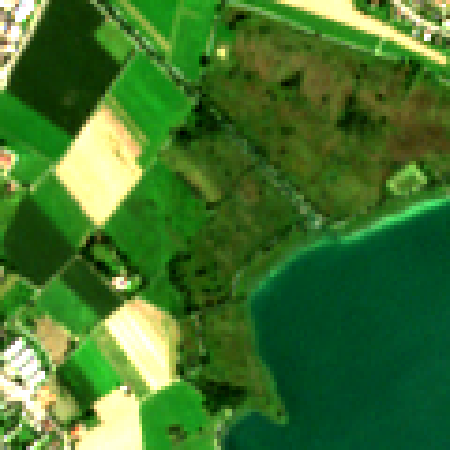
\includegraphics[width=\BenImgWidth]{figures/dataset/samples/_tci_S2A_MSIL2A_20170818T103021_N9999_R108_T32TMT_61_44.png}};
        \end{scope}
        \begin{scope}
          % \clip[rounded corners=5mm]
          %   ($(\rOuter, \rOuter) + (0,.1)$)
          %   rectangle
          %   ($(\rOuter, \rOuter)+(\BenImgWidth, \BenImgWidth) + (0,.1)$);
        
          \node[anchor=south west, inner sep=0pt] at ($(\rOuter, \rOuter) + (0,.1)$)
            {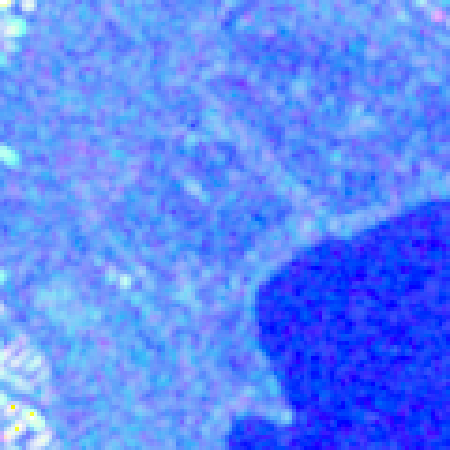
\includegraphics[width=\BenImgWidth]{figures/dataset/samples/_rtc_S2A_MSIL2A_20170818T103021_N9999_R108_T32TMT_61_44.png}};
        \end{scope}
    \end{tikzpicture} 

    \caption{\bentxt{} comprises \num{464 044} co-registered \ac{S1} and \ac{S2} images with diverse text annotations, resulting in a total of $\sim~\num{9.6}$ million \ac{S1}-\ac{S2}-text triplets. The dataset supports 15 tasks (Presence, Area, Counting, Adjacency, Relative Position, Country, Season, and Climate Zone, denoted as \presenceABBR, \areaABBR, \countABBR, \adjacencyABBR, \relativepositionABBR, \countryABBR, \seasonABBR, and \climateABBR, respectively) across 4 broad categories.}
    \label{fig:dataset_overview}
\end{figure*}
Unprecedented advances in satellite technology have led to a significant increase in the volume of \ac{EO} data archives (\eg the Sentinel satellites of the Copernicus program alone acquire roughly 20~TB of satellite images per day).
In this data-rich landscape, natural language provides an intuitive interface for querying and interpreting these vast \ac{EO} archives, with \acp{VLM} emerging as an effective framework for jointly encoding visual observations and natural language for tasks such as image captioning~\cite{cheng2022nwpu, hoxha2020toward, sumbul2020sd}, \ac{VQA}~\cite{lobry2020rsvqa, chappuis2022prompt, hackel2023lit} and \genDet~\cite{kuckreja2024geochat, soni2025earthdial, zhan2025skyeyegpt}.

In general, \acp{VLM} are applied to \ac{EO} data either by using general-purpose \ac{CV} \acp{VLM} directly or by training \ac{RS}-specific \acp{VLM}.
The first approach is limited by the fundamentally different spectral and spatial characteristics between the \ac{CV} and \ac{RS} images. For example, the \ac{S2} \ac{MS} images comprise 13 spectral bands associated with varying spatial resolutions, while those in \ac{CV} include \ac{RGB} bands in general. The high spectral resolution data enable the discrimination of complex \ac{LULC} classes in RS. Although \ac{RGB} information may be sufficient to distinguish generic classes, \eg,\enquote{Water} from \enquote{Forests and seminatural areas}, additional spectral information beyond the visible spectrum is needed to differentiate complex \ac{LULC} classes, \eg, \enquote{Mixed forest} vs. \enquote{Coniferous forest}~\cite{sumbul2019bigearthnet}. Due to their pretraining phase using \ac{RGB}-only image-text data, the \acp{VLM} in \ac{CV} have limited capability to effectively query and interpret RS data. Although several \ac{RS}-specific \acp{VLM} trained on \ac{RS} image-text datasets~\cite{bazi2024rsllava, zhan2025skyeyegpt, kuckreja2024geochat, muhtar2024lhrs} have recently been developed, most of these models are still trained only on \ac{RGB} data and thus subject to the above-mentioned limitations. It is worth noting that there are only a few works that include multispectral or multi-sensor (e.g., multispectral, \ac{SAR})  image-text data during pre-training~\cite{shu2025earthmind, soni2025earthdial}. The use of multi-sensor data is particularly crucial, since different satellite sensors have the capability of measuring different physical properties of \ac{LULC} classes and their joint use can improve task performance ~\cite{sumbul2021bigearthnet, hong2020more, Sumbul_2025_ICCV}.
However, as shown in \cref{tab:existing_datasets_properties}, the existing \ac{RS} image-text datasets suffer from: i) limited availability of co-registered multi-sensor data that includes more than three bands, and ii) limited diversity in text annotation types.
These limitations directly hinder the ability of \acp{VLM} to characterize: 1) the complex spatial/spectral content of \ac{RS} images; and also 2) complementary information among multi-sensor data. 
 \begin{table*}[h!tb]
    \centering
    %\small
    \renewcommand{\arraystretch}{\arrayStretchFactor}
    \setlength\tabcolsep{1pt}
    \caption{
    Comparison of existing \ac{RS} image-text datasets. Datasets are compared in terms of: 1) the presence of co-registered multi-sensor imagery exceeding three spectral bands; 2) methods used for text annotation, including the presence of an extensive manual quality check (QC); 3) supported tasks; 4) availability of geolocation data and 5) the number of image-text (IT) samples. 
    \rcmark{} indicates that only parts of the dataset fulfill this property.
    }
    \begin{tabular}{l >{\centering\arraybackslash}p{0.5cm} >{\centering\arraybackslash}p{0.8cm} >{\centering\arraybackslash}p{0.5cm} c >{\centering\arraybackslash}p{0.5cm} >{\centering\arraybackslash}p{0.5cm} >{\centering\arraybackslash}p{0.5cm} >{\centering\arraybackslash}p{0.5cm} >{\centering\arraybackslash}p{0.5cm} c >{\centering\arraybackslash}p{0.5cm} >{\centering\arraybackslash}p{0.5cm} >{\centering\arraybackslash}p{0.8cm} c r}
    \toprule
     \multirow{2}{*}{\makecell{\\[14pt]Dataset}}     & \multicolumn{3}{c}{\makecell{Multi-Sensor\\[-4pt]Images}} && \multicolumn{5}{c}{Annotation Method} && \multicolumn{3}{c}{\makecell{Supported\\[-4pt]Tasks}} & \multirow{2}{*}{\rb{Geolocation data\gap{8pt}}} & \multirow{2}{*}{\rb{\#IT samples\gap{7pt}}}\\
     \cmidrule{2-4} \cmidrule{6-10} \cmidrule{12-14}
                                                     & \multicolumn{1}{c}{\rb{Available}} & \multicolumn{1}{c}{\rb{\makecell{>3 bands\\[-4pt]per image}}} & \multicolumn{1}{c}{\rb{Co-registered}} && \multicolumn{1}{c}{\rb{Manual}} & \multicolumn{1}{c}{\rb{Template}} & \multicolumn{1}{c}{\rb{Web scraped}} & \multicolumn{1}{c}{\rb{LLM-based}} & \multicolumn{1}{c}{\rb{Manual QC}} && \multicolumn{1}{c}{\rb{Captioning}} & \multicolumn{1}{c}{\rb{VQA}} & \multicolumn{1}{c}{\rb{\makecell{Ref. Exp.\\[-4pt]Detection}}}\\
\midrule
                                                     % ms-avail  all-bands ms-paired   manual   template  web       llm       manual-qc  captioning vqa      det       loc      samples
     UCM-Captions~\cite{qu2016deep}                  & \rxmark & \rxmark & \rxmark && \gcmark & \rxmark & \rxmark & \rxmark & \gcmark && \gcmark & \rxmark & \rxmark & \rxmark & 10.5k \\
     Sydney-Captions~\cite{qu2016deep}               & \rxmark & \rxmark & \rxmark && \gcmark & \rxmark & \rxmark & \rxmark & \gcmark && \gcmark & \rxmark & \rxmark & \rxmark & 3k \\
     RSICD~\cite{lu2017exploring}                    & \rxmark & \rxmark & \rxmark && \gcmark & \rxmark & \rxmark & \rxmark & \gcmark && \gcmark & \rxmark & \rxmark & \rxmark & 54.6k \\
     RSITMD~\cite{yuan2022exploring}                 & \rxmark & \rxmark & \rxmark && \gcmark & \rxmark & \rxmark & \rxmark & \gcmark && \gcmark & \rxmark & \rxmark & \rxmark & 23.7k \\
     NWPU-Captions~\cite{cheng2022nwpu}              & \gcmark & \rxmark & \rxmark && \gcmark & \rxmark & \rxmark & \rxmark & \gcmark && \gcmark & \rxmark & \rxmark & \rxmark & 157k \\
     GAIA~\cite{gaia_zavras}                         & \gcmark & \rxmark & \rxmark && \rxmark & \rxmark & \gcmark & \gcmark & \rxmark && \gcmark & \rxmark & \rxmark & \rcmark & 205k \\
     Git-10M~\cite{Text2Earth_git_10m}               & \gcmark & \rxmark & \rxmark && \rxmark & \rxmark & \rxmark & \gcmark & \rxmark && \gcmark & \rxmark & \rxmark & \gcmark & 10.5M \\
     RSVQAxBEN~\cite{lobryRSVQAMeetsBigearthnet2021} & \rxmark & \rxmark & \rxmark && \rxmark & \gcmark & \rxmark & \rxmark & \rxmark && \rxmark & \gcmark & \rxmark & \rxmark & 14.8M \\
     RS5M~\cite{zhang2024rs5m}                       & \gcmark & \rxmark & \rxmark && \rxmark & \rxmark & \rcmark & \rcmark & \rxmark && \gcmark & \rxmark & \rxmark & \rcmark & 5.0M \\
     RSTeller~\cite{ge2025rsteller}                  & \rxmark & \rxmark & \rxmark && \rxmark & \rxmark & \rxmark & \gcmark & \rxmark && \gcmark & \rxmark & \rxmark & \rxmark & 2.6M \\
     Landsat30-AU~\cite{ma2025landsat30}             & \rxmark & \rxmark & \rxmark && \rxmark & \rxmark & \rxmark & \gcmark & \rcmark && \gcmark & \gcmark & \rxmark & \rcmark & 216k \\
     ChatEarthNet~\cite{ChatEarthNet}                & \rxmark & \gcmark & \rxmark && \rxmark & \rxmark & \rxmark & \gcmark & \rcmark && \gcmark & \rxmark & \rxmark & \rxmark & 173k \\
     MS-Clip~\cite{marimo2025beyond}                 & \gcmark & \gcmark & \gcmark && \rxmark & \rxmark & \rxmark & \gcmark & \rxmark && \gcmark & \rxmark & \rxmark & \rxmark & 985k \\
     \bentxt (ours)                                  & \gcmark & \gcmark & \gcmark && \rxmark & \gcmark & \rxmark & \gcmark & \rcmark && \gcmark & \gcmark & \gcmark & \gcmark & 9.6M \\
    \bottomrule
    \end{tabular}
    \label{tab:existing_datasets_properties}
\end{table*}

To overcome the above-mentioned limitations, in this paper we present \bentxt: a large-scale image-text dataset made up of \num{464044} co-registered \acl{S1} \acl{SAR} and \acl{S2} \acl{MS} images with \SI{9.6}{\mega\nothing} text annotations, including captions, \acp{VQA} with varying answer formats, and \genDet{} annotations (see \cref{fig:dataset_overview}). In addition, we introduce a \bench{} that contains \num{1082} image pairs with manually verified text annotations for systematic evaluation of VLMs for EO tasks. Using our \bench{}, we demonstrate that current \acp{VLM} in both \ac{CV} and \ac{RS} show limited ability to characterize the complex content of multi-sensor \ac{RS} images. Fine-tuning a \ac{SOTA} \ac{VLM} (InternVL3-1B~\cite{zhu2025internvl3}) adapted for multi-sensor input (denoted as RS-InternVL) on \bentxt{} leads to substantial performance gains across all considered tasks.

In summary, our contributions are as follows:
\begin{enumerate}
    \item We show that the existing \acp{VLM} from both \ac{CV} and \ac{RS} domains exhibit limited capability to characterize the complex spatial/spectral content of multi-sensor images in \ac{RS}. To this end, we conduct extensive experiments across 15 tasks of 4 categories: image captioning, binary \ac{VQA}, \ac{MCQ}, and \genDet.
    \item We introduce \bentxt{} (which is the first dataset unifying co-registered multi-sensor \ac{RS} data with diverse textual descriptions) together with a manually checked subset (\bench{}).
    \item We adapt InternVL to accommodate multi-sensor RS inputs and perform domain-specific fine-tuning using \bentxt. Our results serve as experimental validation of the critical role of large-scale, multi-sensor image-text datasets for accurate interactions with EO data.
\end{enumerate}